\clearpage
\section{Microbiome DNA 16S}

\subsubsection{Pcaplot}
\begin{figure}[h]
\centering
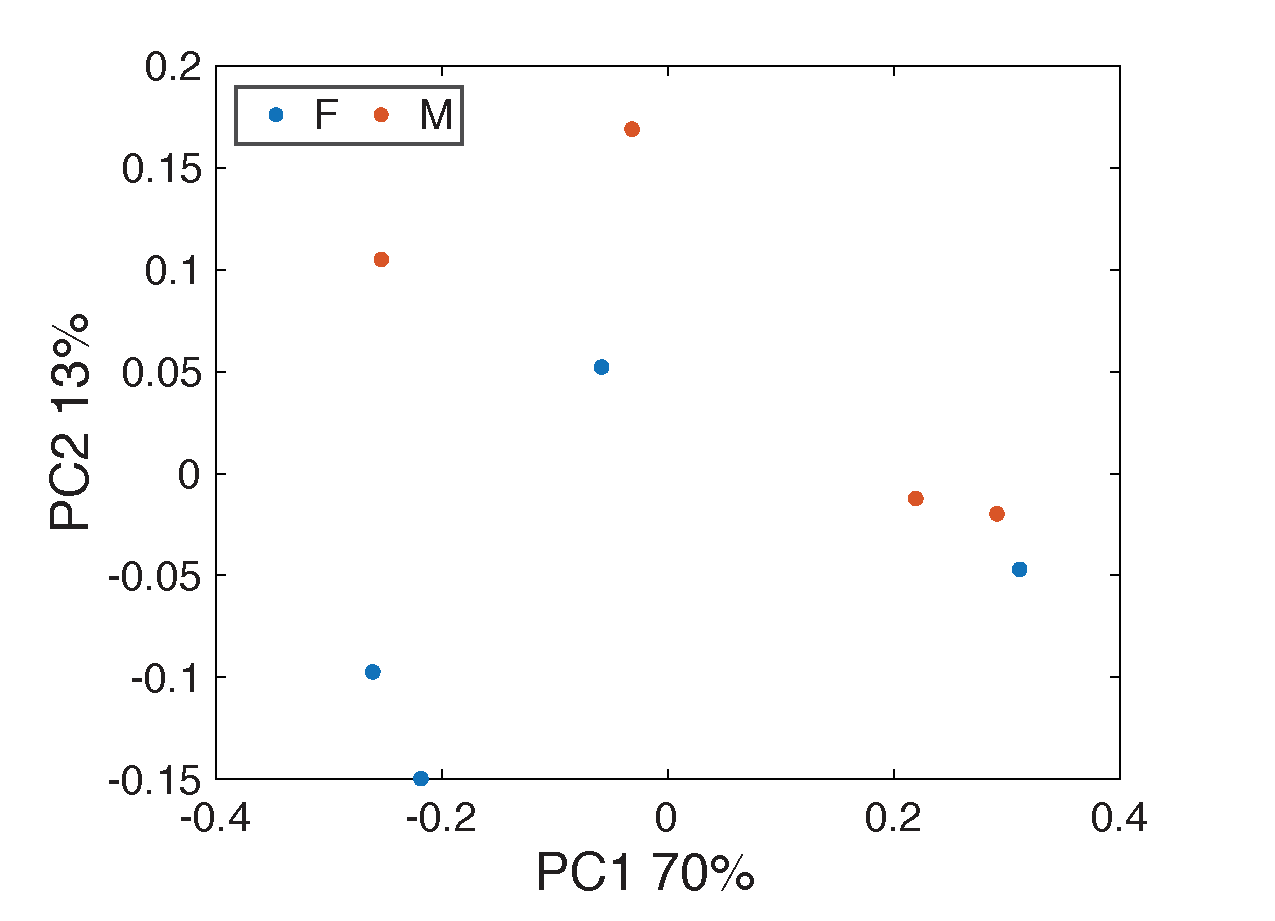
\includegraphics[width=.6\textwidth]{../30_tissue_supplement_figures/Microbiome/dna_16s/Microbiome_mouse-sex_pcaplot.pdf}

\caption{Principal Coordinate Analysis shows that the composition and beta diversity does not separate based on gender.}
\end{figure}


\clearpage

\subsubsection{Barplot}
\begin{figure}[h]
\centering
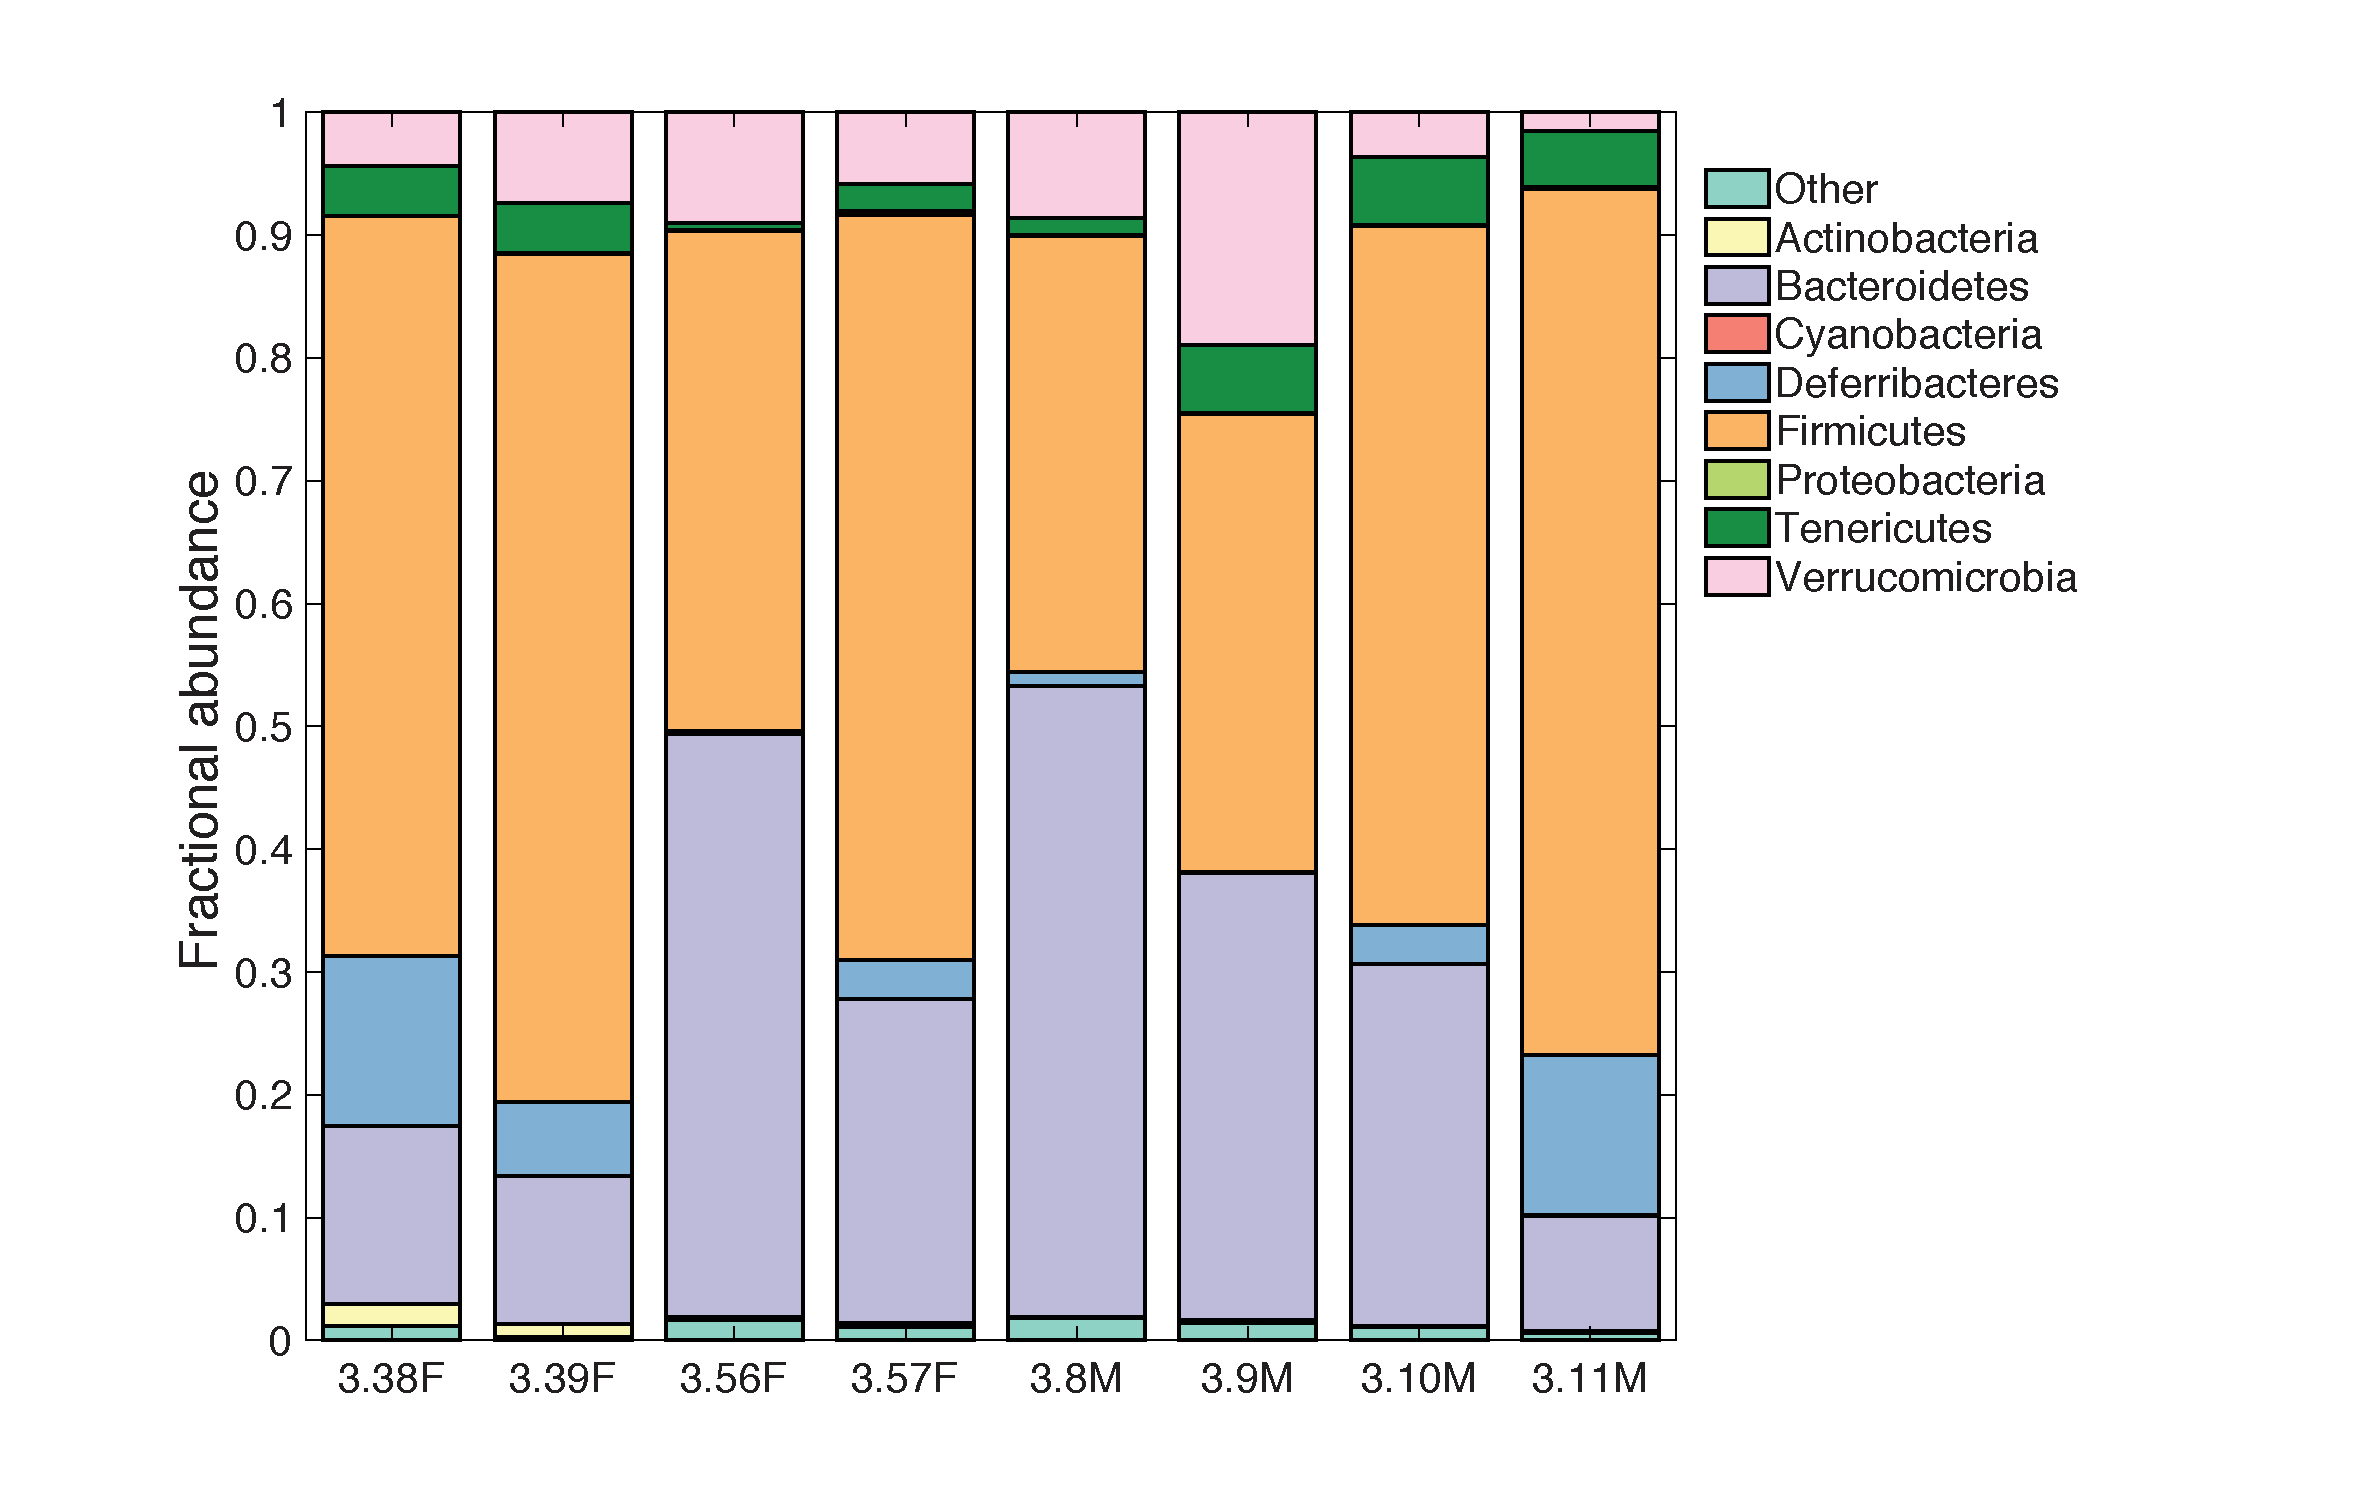
\includegraphics[width=.6\textwidth]{../30_tissue_supplement_figures/Microbiome/dna_16s/Microbiome_taxa_barplot.pdf}

\caption{Taxonomic variation in the mouse gut microbiome. Relative abundance of bacterial phyla across 8 faecal microbiomes. F indicates female mice, M indicates males.
}
\end{figure}

